\documentclass[letterpaper,USenglish,cleveref, autoref, thm-restate]{lipics-v2021}
%This is a template for producing LIPIcs articles.
%See lipics-v2021-authors-guidelines.pdf for further information.
%for A4 paper format use option "a4paper", for US-letter use option "letterpaper"
%for british hyphenation rules use option "UKenglish", for american hyphenation rules use option "USenglish"
%for section-numbered lemmas etc., use "numberwithinsect"
%for enabling cleveref support, use "cleveref"
%for enabling autoref support, use "autoref"
%for anonymousing the authors (e.g. for double-blind review), add "anonymous"
%for enabling thm-restate support, use "thm-restate"
%for enabling a two-column layout for the author/affilation part (only applicable for > 6 authors), use "authorcolumns"
%for producing a PDF according the PDF/A standard, add "pdfa"

%\pdfoutput=1 %uncomment to ensure pdflatex processing (mandatatory e.g. to submit to arXiv)
%\hideLIPIcs  %uncomment to remove references to LIPIcs series (logo, DOI, ...), e.g. when preparing a pre-final version to be uploaded to arXiv or another public repository

%\graphicspath{{./graphics/}}%helpful if your graphic files are in another directory

\usepackage{amsmath}
\usepackage{amssymb}
\usepackage{tikz}
\usepackage{pgfplots}
\usepackage{booktabs}
\usepackage{hyperref}

\newcommand{\pand}{\mathbin{\land^\textsf{p}}}
\newcommand{\por}{\mathbin{\lor^\textsf{p}}}
\DeclareMathOperator*{\Pand}{\bigwedge^\textsf{p}}
\DeclareMathOperator*{\Por}{\bigvee^\textsf{p}}
\newcommand{\boolnot}{\neg}
\newcommand{\tautology}{\top}
\newcommand{\nil}{\bot}
\newcommand{\obar}[1]{\overline{#1}}
\newcommand{\oneminus}{{\sim}}
\newcommand{\lit}{\ell}

\newcommand{\varset}{X}
\newcommand{\exvarset}{Z}
\newcommand{\dependencyset}{{\cal D}}
\newcommand{\litset}{{\cal L}}
\newcommand{\ring}{{\cal R}}
\newcommand{\dset}{{\cal A}}
\newcommand{\rep}{\textbf{R}}
\newcommand{\radd}{+}
\newcommand{\rmul}{\times}
\newcommand{\addident}{\textbf{0}}
\newcommand{\mulident}{\textbf{1}}
\newcommand{\imply}{\Rightarrow}
\newcommand{\ifandonlyif}{\Leftrightarrow}
%\newcommand{\drational}{\mathbb{Q}_{2,5}}
\newcommand{\drational}{\textbf{Q}_{2,5}}
\newcommand{\entail}{\vDash}
\newcommand{\entaildrat}{\entail_{\textrm{DRAT}}}

\newcommand{\assign}{\alpha}
\newcommand{\passign}{\rho}
\newcommand{\lassign}{\beta}
\newcommand{\uassign}{{\cal U}}
\newcommand{\modelset}{{\cal M}}

\newcommand{\indegree}{\textrm{indegree}}
\newcommand{\outdegree}{\textrm{outdegree}}
\newcommand{\validate}{\textsf{validate}}
\newcommand{\prov}{\textrm{Prov}}
\newcommand{\inputformula}{\phi_I}
\newcommand{\pogformula}{\theta_P}

\newcommand{\makenode}[1]{\mathbf{#1}}
\newcommand{\nodeu}{\makenode{u}}
\newcommand{\nodev}{\makenode{v}}
\newcommand{\nodes}{\makenode{s}}
\newcommand{\nodep}{\makenode{p}}
\newcommand{\noder}{\makenode{r}}

\newcommand{\simplify}[2]{#1|_{#2}}

\newcommand{\progname}[1]{\textsc{#1}}
\newcommand{\dfour}{\progname{D4}}
\newcommand{\cdfour}{\progname{CD4}}
\newcommand{\Dfour}{\progname{D4}}
\newcommand{\cadical}{\progname{CaDiCal}}
\newcommand{\dtrim}{\progname{drat-trim}}
\newcommand{\Dtrim}{\progname{Drat-trim}}

\definecolor{redorange}{rgb}{0.878431, 0.235294, 0.192157}
\definecolor{lightblue}{rgb}{0.552941, 0.72549, 0.792157}
\definecolor{clearyellow}{rgb}{0.964706, 0.745098, 0}
\definecolor{clearorange}{rgb}{0.917647, 0.462745, 0}
\definecolor{mildgray}{rgb}{0.54902, 0.509804, 0.47451}
\definecolor{softblue}{rgb}{0.643137, 0.858824, 0.909804}
\definecolor{bluegray}{rgb}{0.141176, 0.313725, 0.603922}
\definecolor{lightgreen}{rgb}{0.709804, 0.741176, 0}
\definecolor{darkgreen}{rgb}{0.152941, 0.576471, 0.172549}
\definecolor{redpurple}{rgb}{0.835294, 0, 0.196078}
\definecolor{midblue}{rgb}{0, 0.592157, 0.662745}
\definecolor{clearpurple}{rgb}{0.67451, 0.0784314, 0.352941}
\definecolor{browngreen}{rgb}{0.333333, 0.313725, 0.145098}
\definecolor{darkestpurple}{rgb}{0.396078, 0.113725, 0.196078}
\definecolor{greypurple}{rgb}{0.294118, 0.219608, 0.298039}
\definecolor{darkturquoise}{rgb}{0, 0.239216, 0.298039}
\definecolor{darkbrown}{rgb}{0.305882, 0.211765, 0.160784}
\definecolor{midgreen}{rgb}{0.560784, 0.6, 0.243137}
\definecolor{darkred}{rgb}{0.576471, 0.152941, 0.172549}
\definecolor{darkpurple}{rgb}{0.313725, 0.027451, 0.470588}
\definecolor{darkestblue}{rgb}{0, 0.156863, 0.333333}
\definecolor{lightpurple}{rgb}{0.776471, 0.690196, 0.737255}
\definecolor{softgreen}{rgb}{0.733333, 0.772549, 0.572549}
\definecolor{offwhite}{rgb}{0.839216, 0.823529, 0.768627}
\definecolor{medgreen}{rgb}{0.15, 0.6, 0.15}

% Lean code:
\usepackage{listings}
%\definecolor{keywordcolor}{rgb}{0.7, 0.1, 0.1}   % red
\definecolor{keywordcolor}{rgb}{0.0, 0.1, 0.6}   % blue
\definecolor{tacticcolor}{rgb}{0.0, 0.1, 0.6}    % blue
\definecolor{commentcolor}{rgb}{0.4, 0.4, 0.4}   % grey
\definecolor{symbolcolor}{rgb}{0.0, 0.1, 0.6}    % blue
\definecolor{sortcolor}{rgb}{0.1, 0.5, 0.1}      % green
\definecolor{attributecolor}{rgb}{0.7, 0.1, 0.1} % red
\def\lstlanguagefiles{lstlean.tex}
% set default language
\lstset{language=lean, xleftmargin=1em}
\lstset{backgroundcolor=\color{white}}

\bibliographystyle{plainurl}% the mandatory bibstyle

\title{Certified Knowledge Compilation \\ with Application to Verified Model Counting}

\titlerunning{Certified Knowledge Compilation}

\author{Randal E. Bryant}{Computer Science Department, Carnegie Mellon University, Pittsburgh, PA 15213 USA}{Randy.Bryant@cs.cmu.edu}{https://orcid.org/0000-0001-5024-6613}{Supported by NSF grant CCF-2108521}
\author{Wojciech Nawrocki}{Department of Philosophy, Carnegie Mellon University}{wjnawrocki@cmu.edu}{https://orcid.org/0000-0002-8839-0618}{Hoskinson Center for Formal Mathematics}
\author{Jeremy Avigad}{Department of Philosophy, Carnegie Mellon University}{avigad@cmu.edu}{https://orcid.org/0000-0003-1275-315X}{Hoskinson Center for Formal Mathematics}
\author{Marijn J. H. Heule}{Computer Science Department, Carnegie Mellon University}{marijn@cmu.edu}{https://orcid.org/0000-0002-5587-8801}{Supported by NSF grant CCF-2108521}

\authorrunning{R. E. Bryant et al.} %TODO mandatory. First: Use abbreviated first/middle names. Second (only in severe cases): Use first author plus 'et al.'

\Copyright{Randal E. Bryant, Wojciech Nawrocki, Jeremy Avigad, and Marijn J. H. Heule} %TODO mandatory, please use full first names. LIPIcs license is "CC-BY";  http://creativecommons.org/licenses/by/3.0/

%\ccsdesc[100]{\textcolor{red}{Replace ccsdesc macro with valid one}} %TODO mandatory: Please choose ACM 2012 classifications from https://dl.acm.org/ccs/ccs_flat.cfm
\begin{CCSXML}
<ccs2012>
   <concept>
       <concept_id>10003752.10003790.10003794</concept_id>
       <concept_desc>Theory of computation~Automated reasoning</concept_desc>
       <concept_significance>500</concept_significance>
       </concept>
 </ccs2012>
\end{CCSXML}

\ccsdesc[500]{Theory of computation~Automated reasoning}


%\keywords{Dummy keyword} %TODO mandatory; please add comma-separated list of keywords
\keywords{Propositional model counting, Proof checking}

%\category{} %optional, e.g. invited paper

%\funding{(Optional) general funding statement \dots}%optional, to capture a funding statement, which applies to all authors. Please enter author specific funding statements as fifth argument of the \author macro.

\nolinenumbers %uncomment to disable line numbering

\EventEditors{Meena Mahajan and Friedrich Slivovsky}
\EventNoEds{2}
\EventLongTitle{26th International Conference on Theory and Applications of Satisfiability Testing (SAT 2023)}
\EventShortTitle{SAT 2023}
\EventAcronym{SAT}
\EventYear{2023}
\EventDate{July 4--8, 2023}
\EventLocation{Alghero, Italy}
\EventLogo{}
\SeriesVolume{271}
\ArticleNo{6}

%Editor-only macros:: begin (do not touch as author)%%%%%%%%%%%%%%%%%%%%%%%%%%%%%%%%%%
%\EventEditors{John Q. Open and Joan R. Access}
%\EventNoEds{2}
%\EventLongTitle{42nd Conference on Very Important Topics (CVIT 2016)}
%\EventShortTitle{CVIT 2016}
%\EventAcronym{CVIT}
%\EventYear{2016}
%\EventDate{December 24--27, 2016}
%\EventLocation{Little Whinging, United Kingdom}
%\EventLogo{}
%\SeriesVolume{42}
%\ArticleNo{23}
%%%%%%%%%%%%%%%%%%%%%%%%%%%%%%%%%%%%%%%%%%%%%%%%%%%%%%

\newcommand{\program}[1]{\textsc{#1}}
\newcommand{\lean}{Lean~4}

\begin{document}

\maketitle

\begin{abstract}

Computing many useful properties of Boolean formulas, such as their weighted or unweighted model count,
is intractable on general representations. It can become tractable when formulas are expressed in a
special form, such as the deterministic,
decomposable, negation normal form (det-DNNF)\@.
\emph{Knowledge compilation} is the process of converting a formula
into such a form. Unfortunately existing knowledge compilers provide no guarantee that their output correctly
represents the original formula, and therefore they cannot validate a model count, or any other computed value.

We present \emph{Partitioned-Operation Graphs} (POGs), a general form that can
encode all
of the representations used by existing knowledge compilers.
We have designed  CPOG, a framework that can express proofs of equivalence between a
POG  and a Boolean formula in conjunctive normal form (CNF).

We have developed a program that generates POG representations from det-DNNF
graphs 
produced by the state-of-the-art knowledge compiler
\dfour{}, as well as checkable CPOG proofs certifying that the output POGs
are equivalent to the input CNF formulas.  Our toolchain
for generating and verifying POGs scales to all but the largest
graphs produced by \dfour{} for formulas from a recent model counting
competition. Additionally, we have developed a formally verified CPOG
checker and model counter for POGs in the \lean{} proof assistant.
In doing so, we proved the soundness of our proof framework. These programs
comprise the first formally verified toolchain for weighted and unweighted
model counting.
\end{abstract}

\section{Introduction}

Given a Boolean formula $\phi$, modern Boolean satisfiability (SAT) solvers can
find an assignment satisfying $\phi$ or generate a proof that no
such assignment exists.  They have applications across a variety of
domains including computational mathematics, combinatorial
optimization, and the formal verification of hardware, software, and
security protocols.  Some applications, however, require going
beyond Boolean satisfiability.  For example, the \emph{model
  counting problem} requires computing the number of satisfying
assignments of a formula, including in cases where there are far too many
to enumerate individually.  Model counting has
applications in artificial intelligence, computer security, and
statistical sampling.  There are also many useful extensions of standard model counting,
including {\em
  weighted model counting}, where a weight is defined for
each possible assignment, and the goal becomes to compute the sum of the weights
of the satisfying assignments.

Model counting is a challenging problem---more challenging than the
already NP-hard Boolean satisfiability.  Several
tractable variants of Boolean satisfiability, including 2-SAT, become
intractable when the goal is to count models and not just determine
satisfiability \cite{valiant:siam:1979}.  Nonetheless, a number of
model counters that scale to very large formulas have been developed, as
witnessed by the progress in recent model counting competitions.

One approach to model counting, known as \emph{knowledge compilation},
transforms the formula into a structured form for which model counting
is straightforward.  For example, the \emph{deterministic
decomposable, negation normal form}
(det-DNNF) introduced by
Darwiche~\cite{darwiche:aaai:2002,darwiche:ecai:2004}
represents a
Boolean formula as a directed acyclic graph, with terminal nodes
labeled by Boolean variables and their complements, and with each
nonterminal node labeled by a Boolean And or Or operation.  Restrictions
are placed on the structure of the graph such that a count of the
models can be computed by a single bottom-up traversal.
Kimmig et al.\ present a very general {\em
  algebraic model counting}~\cite{kimmig:jal:2017} framework describing
properties of Boolean functions that can be efficiently computed from
a det-DNNF representation.  These include standard and weighted model
counting, and much more.

One shortcoming of existing knowledge compilers is that they have no
generally accepted
way to validate that their generated results are correct, i.e., that
the compiled representation is logically equivalent to the original
formula.  By contrast, all modern SAT solvers can generate
checkable proofs when they encounter unsatisfiable formulas.  The
guarantee provided by a checkable certificate of correctness enables
users of SAT solvers to fully trust their results.  Experience has also
shown that proof production capabilites allow SAT solver developers to quickly
detect and diagnose bugs in their programs. This, in turn, has led
to more reliable SAT solvers.

This paper introduces \emph{Partitioned-Operation Graphs} (POGs),
a general form that can encode all of the representations produced by current knowledge
compilers. The CPOG (for ``certified'' POG) file format then
captures both the structure of a POG
and a checkable proof of its logical equivalence to a Boolean formula in
conjunctive normal form (CNF).  A CPOG
proof consists of a sequence of clause addition and deletion steps,
based on an extended resolution proof system~\cite{Tseitin:1983}.
We establish a set of conditions that, when satisified by a CPOG file, guarantees that it
encodes a well-formed POG and provides a valid equivalence proof.

\begin{figure}
\centering{
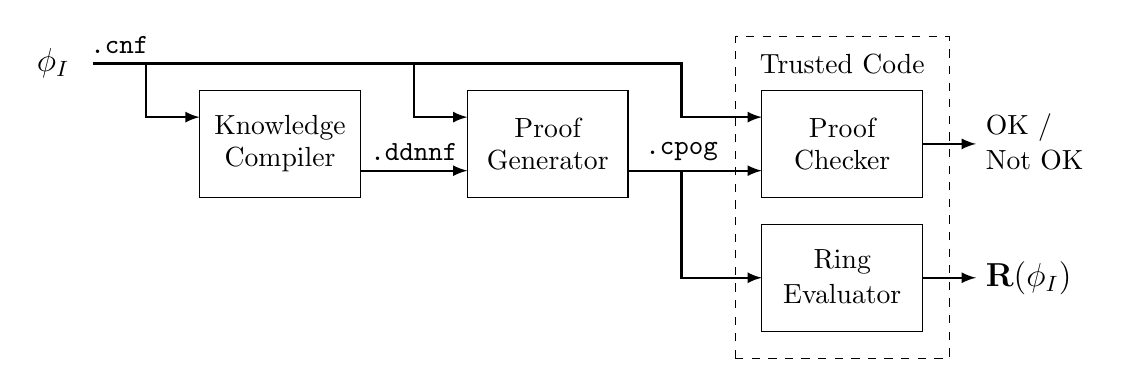
\begin{tikzpicture}[scale=0.17]
  \draw (8,10) rectangle (20,18);
  \node at (14,15.2) {Knowledge};
  \node at (14,12.8) {Compiler};

  \draw (28,10) rectangle (40,18);
  \node at (34,15.2) {Proof};
  \node at (34,12.8) {Generator};


  \draw (50,10) rectangle (62,18);
  \node at (56,15.2) {Proof};
  \node at (56,12.8) {Checker};

  \draw (50,0) rectangle (62,8);
  \node at (56,5.2) {Ring};
  \node at (56,2.8) {Evaluator};

  \draw[dashed] (48,-2) rectangle (64,22);
  \node at (56,20) {Trusted Code};

  %% CNF
  \draw[thick] (0,20) -- (44,20) -- (44,16) [-latex] -- (50,16);
  \draw[thick] (4,20) -- (4,16) [-latex] -- (8,16);
  \draw[thick] (24,20) -- (24,16) [-latex] -- (28,16);
  \node [left] at (-1,20) {\large {$\inputformula$}};
  \node [above] at (2,20) {\texttt{.cnf}};

  %% NNF
  \draw[thick] (20,12) [-latex] -- (28,12);
  \node [above] at (24,12) {\texttt{.ddnnf}};

  %% CPOG
  \draw[thick] (40,12) [-latex] -- (50,12);
  \draw[thick] (44,12) -- (44,4) [-latex] -- (50,4);
  \node [above] at (44,12) {\texttt{.cpog}};

  %% OK/Not
  \draw[thick] (62,14) [-latex] -- (66,14) ;
  \node [right] at (66,15.2) { OK /} ;
  \node [right] at (66,12.8) { Not OK} ;
  \draw[thick] (62,4) [-latex] -- (66,4) ;
  \node [right] at (66,4) {\large {$\textbf{R}(\inputformula)$}};

\end{tikzpicture}
}
\caption{Certifying toolchain.
  The output of a standard knowledge compiler is converted into a combined graph/proof (CPOG)
  which can be independently checked and evaluated}
\label{fig:chain}
\end{figure}

Figure~\ref{fig:chain} illustrates our certifying knowledge
compilation and model counting toolchain.  Starting with
input formula $\inputformula$, the \dfour{} knowledge compiler~\cite{lagniez:ijcai:2017}
generates a \emph{decision} DNNF (dec-DNNF) representation (a restricted form of det-DNNF),
and the \emph{proof
  generator} uses this to generate a CPOG file.
The \emph{proof checker} verifies the equivalence of the CNF and CPOG representations.
The \emph{ring evaluator} computes
a standard or weighted model count from the POG\@ representation.
As the dashed box in Figure~\ref{fig:chain} indicates, this toolchain
moves the root of trust away from the complex and highly
optimized knowledge compiler to a relatively simple checker and
evaluator.  Importantly, the proof generator need not be
trusted---its errors will be caught by the proof checker.

To ensure soundness of the abstract CPOG proof system, as well as
correctness of its concrete implementation, we formally verified the
proof system as well as versions of the proof checker and ring
evaluator in the \lean{} proof assistant~\cite{demoura:cade:2021}.
Running these two programs on a particular CPOG file gives strong
assurance that the proof and the model count are correct. Our
experience with developing a formally verified proof checker has shown
that, even within the well-understood framework of extended
resolution, it can be challenging to formulate a full set of
requirements that guarantee soundness.  In fact, our efforts to
formally verify our proof framework exposed subtle conditions that we had
to impose on our partitioned sum rule.

We evaluate our toolchain using benchmark formulas from the 2022
standard and weighted model competitions.  Our tools handle all but
the largest dec-DNNF graphs generated by \dfour{}.  We also measure
the benefits of several optimizations as well as the relative
performance of the verified checker with one designed for high
performance and capacity.  We also show that our tools can provide
end-to-end verification of formulas that have been transformed by an
equivalence-preserving preprocessor.

We have developed an online supplement to this
paper~\cite{bryant:sat:2023:supplement} containing additional
information, including a worked example, details on the algorithms,
and extensive experimental results.  The archive also includes copies
of the programs and a set of benchmark files for testing.


\section{Related Work}


Generating proofs of unsatisfiability in SAT solvers has a long
tradition~\cite{ZhangMalik} and has become widely accepted due to the
formulation of clausal proof systems for which proofs can readily be
generated and efficiently checked
\cite{RAT,wetzler14_drattrim}.
A number of formally verified checkers have been developed within different verification frameworks~\cite{cruz-cade-2017,lrat,Lammich:20,Tan:2021}.
The associated proofs add clauses while preserving satisfiability until the empty clause is derived.
Our work builds on the well-established technology and tools associated with clausal proof systems,
but we require features not found in proofs of unsatisfiability.
Our proofs construct a new propositional formula, and we must verify
%both
that it
%satisfies a set of rules and that it
is equivalent to the input formula.  This requires verifying
additional proof steps, including clause deletion steps, and subtle
invariants, as described in Sections~\ref{sect:cpog} and
\ref{section:formally-verified-toolchain}.

Capelli et al.\ developed a knowledge compiler
that generates a certificate in a proof system that is itself based on
dec-DNNF~\cite{capelli:sat:2019,capelli:aaai:2021}.  Their \cdfour{} program,
a modified version of \dfour{}, generates annotations to the
compiled representation, providing information about how the compiled version relates to the input clauses.
It also generates a file of clausal proof steps in the DRAT format~\cite{wetzler14_drattrim}.
Completing the certification involves running two different checkers on
the annotated dec-DNNF graph and the DRAT file.
Although the authors make informal arguments
regarding the soundness of their frameworks, these do not provide
strong levels of assurance.  Indeed, 
we have identified a weakness in the their
methodology due to an invalid assumption about the
guarantees provided by \dtrim{}, the program it uses to check the
DRAT file.

In more detail, \cdfour{} emits a sequence of clauses $R$ that
includes the conflict clauses that arose via a top-down processing of
the input clauses.  Given input formula $\phi$, their first task is to
check whether $\phi \imply R$, i.e., that any assignment that satisfies $\phi$ also satisfies each of the clauses in $R$.
They then base other parts of their proof on that
property and use a separate checker to perform a series of additional
checks.  They use \dtrim{} to prove the implication, checking that each clause in $R$
satisifies the \emph{reverse asymmetric tautology} (RAT) property with
respect to the preceding
clauses~\cite{heule:cade:2013,jarvisalo:ijcar:2012}.  Adding a RAT
clause $C$ to a set of clauses maintains satisfiability, but it may
not preserve models.  As an example, consider the following formulas:
\begin{center}
  \begin{tabular}{lccc}
    $\phi_1$: & $(x_1 \lor x_3)$ & & \\
    $\phi_2$: & $(x_1 \lor x_3)$ & $\land$ & $(x_1 \lor \obar{x}_2)$\\    
  \end{tabular}
\end{center}
Clearly, these two formulas are not equivalent---$\phi_1$ has six
models, while $\phi_2$ has five.  In particular, $\phi_1$ allows
arbitrary assignments to variable $x_2$.  Critically, however the
second clause of $\phi_2$ is RAT with respect to the first---any
satisfying assignment to $\phi_1$ can be transformed into one that
also satisfies $\phi_2$ by setting $x_2 = 0$.
  
This weakness would allow a buggy (or malicious) version
of \cdfour{} to generate a compiled representation of $\phi_2$ when
given $\phi_1$ as its input.  By adding the second clause to $R$,
the check with \dtrim{} would pass, as would the other tests performed
by their checker.  We have been able to confirm this possibility with
their compiler and checker\footnote{Downloaded May 18, 2023 as\\
\url{https://github.com/crillab/d4/tree/333370cc1e843dd0749c1efe88516e72b5239174}.}


This weakness can be corrected by restricting \dtrim{} to only add
clauses that obey the stronger \emph{reverse unit propagation} (RUP) property~\cite{goldberg,vangelder08_verifying_rup_proofs}.  We have added a
commandline argument to \dtrim{}\footnote{Available at
\url{https://github.com/marijnheule/drat-trim/tree/develop}.} that enforces this
restriction.  This weakness, however, illustrates the general challenge of
developing a new proof framework.
Without a formal verification, there are likely to be 
conditions that make the framework unsound.

Fichte, Hecher, and Roland~\cite{fichte:sat:2022} devised the MICE
proof framework for model counting programs.  Their proof rules are
based on the algorithms commonly used by model counters.  They
developed a program that can generate proof traces from dec-DNNF
graphs and a program to check adherence to their proof rules.  This
framework is not directly comparable to ours, since it only certifies
the unweighted model count, but it has similar goals.
Again, they provide only  informal arguments 
regarding the soundness of their frameworks.

Both of these prior certification frameworks are strongly tied to the
algorithms used by the knowledge compilers and model counters.  Some
of the conditions to be checked are relevant only to specific
implementations.    Our framework is very general and is based on a small set
of proof rules.  It builds on the highly developed
concepts of clausal proof systems.  These factors were important in enabling formal verification.
In the supplement~\cite{bryant:sat:2023:supplement},
we also compare the performance of our toolchain to these two others.


\section{Logical Foundations}
\label{section:logical:foundations}

  Let $\varset$ denote a set of Boolean variables, and let $\assign$
  be an \emph{assignment} of truth values to some subset of the
  variables, where $0$ denotes false and $1$ denotes true, i.e.,
  $\assign \colon \varset' \rightarrow \{0,1\}$ for some $\varset'
  \subseteq \varset$.  We say the assignment is \emph{total} when it
  assigns a value to every variable ($\varset' = \varset$), and that
  it is \emph{partial} otherwise.
  The set of all possible total assignments over
  $\varset$ is denoted $\uassign$.

For each variable $x \in \varset$,
  we define the \emph{literals} $x$ and $\obar{x}$, where $\obar{x}$ is the
  negation of $x$. An
  assignment $\assign$ can be viewed as a set of literals, where
  we write $\lit \in \assign$ when $\lit = x$ and $\assign(x) = 1$ or when
  $\lit = \obar{x}$ and $\assign(x) = 0$.  We write the negation of literal $\lit$ as $\obar{\lit}$.  That is, $\obar{\lit} = \obar{x}$ when $\lit = x$ and
$\obar{\lit} = x$ when $\lit = \obar{x}$.


\begin{definition}[Boolean Formulas]
  The set of Boolean formulas is defined recursively.  Each
  formula $\phi$ has an associated \emph{dependency set}
  $\dependencyset(\phi)  \subseteq \varset$, and a set of models $\modelset(\phi)$,
  consisting of total assignments that satisfy the formula:
  \begin{enumerate}
  \item Boolean constants $0$ and $1$ are Boolean formulas,
    with $\dependencyset(0) = \dependencyset(1) = \emptyset$, with $\modelset(0) = \emptyset$, and with $\modelset(1) = \uassign$.
  \item Variable $x$ is a Boolean formula, with $\dependencyset(x) = \{x\}$
    and $\modelset(x) = \{\assign \in \uassign | \assign(x)=1\}$.
  \item For formula $\phi$, its \emph{negation}, written $\boolnot \phi$ is a Boolean formula,
    with $\dependencyset(\boolnot \phi) = \dependencyset(\phi)$ and $\modelset(\boolnot \phi) = \uassign - \modelset(\phi)$.
  \item For formulas $\phi_1, \phi_2, \ldots, \phi_k$, their \emph{product} $\phi = \bigwedge_{1 \leq i \leq k} \phi_i$ is a Boolean formula, with
      $\dependencyset(\phi) = \bigcup_{1 \leq i \leq k} \dependencyset(\phi_i)$ and
      $\modelset(\phi) = \bigcap_{1 \leq i \leq k} \modelset(\phi_i)$.
  \item For formulas $\phi_1, \phi_2, \ldots, \phi_k$, their \emph{sum} $\phi = \bigvee_{1 \leq i \leq k} \phi_i$ is a Boolean formula, with
      $\dependencyset(\phi) = \bigcup_{1 \leq i \leq k} \dependencyset(\phi_i)$ and
      $\modelset(\phi) = \bigcup_{1 \leq i \leq k} \modelset(\phi_i)$.
  \end{enumerate}
\label{def:boolean}
\end{definition}


  We highlight two special classes of Boolean formulas.  A formula is
  in \emph{negation normal form} when negation is applied only to variables.  A
  formula is in \emph{conjunctive normal form} (CNF) when i) it is in
  negation normal form, and ii) sum is applied only to literals.  A CNF
  formula can be represented as a set of \emph{clauses}, each of which is a
  set of literals.  Each clause represents the sum of the
  literals, and the formula is the product of its clauses.  We use
  set notation to reference the clauses within a formula and the
  literals within a clause.  A clause consisting of a single literal is referred to as a \emph{unit} clause and the literal as a \emph{unit} literal.
This literal must be assigned value $1$ by any satisfying assignment of the formula.

\begin{definition}[Partitioned-Operation Formula]\label{def:partitioned-operation-formula}
  A \emph{partitioned-operation formula}
 satisfies the following for all product and sum operations:
      \begin{enumerate}
      \item The arguments to each product must have disjoint dependency sets.  That is, operation
        $\bigwedge_{1 \leq i \leq k} \phi_i$ requires $\dependencyset(\phi_i) \cap \dependencyset(\phi_j) = \emptyset$ for $1 \leq i < j \leq k$.
      \item The arguments to each sum must have disjoint models.  That is, operation
        $\bigvee_{1 \leq i \leq k} \phi_i$ requires $\modelset(\phi_i) \cap \modelset(\phi_j) = \emptyset$ for $1 \leq i < j \leq k$.
      \end{enumerate}
\end{definition}
     We let $\pand$ and $\por$ denote the product and sum operations in a partitioned-operation formula.

  \section{Ring Evaluation of a Boolean Formula}

We propose a general framework for summarizing properties of Boolean
formulas along the lines of algebraic model counting~\cite{kimmig:jal:2017}.

\begin{definition}[Commutative Ring]
  A \emph{commutative ring} $\ring$ is an algebraic structure
  $\langle \dset, \radd, \rmul, \addident, \mulident \rangle$,
  with elements in the set $\dset$ and with commutative and
  associative operations $\radd$ (addition) and $\rmul$ (multiplication),
  such that multiplication distributes
  over addition.  $\addident$ is the additive identity and $\mulident$ is
  the multiplicative identity.  Every element $a \in \dset$ has an
  \emph{additive inverse} $-a$ such that $a + -a = \addident$.
\label{def:ring}
\end{definition}
We write $a - b$ as a shorthand for $a + -b$.

\begin{definition}[Ring Evaluation Problem]
\label{def:ring_evaluation}
  For commutative ring $\ring$, a \emph{ring weight function} associates a value $w(x) \in \dset$ with
  every variable $x \in \varset$.  We then define $w(\obar{x}) \doteq \mulident-w(x)$.

  For Boolean formula $\phi$ and ring weight function $w$, the \emph{ring evaluation problem} computes
  \begin{equation}
    \begin{array}{rcl}
    \rep(\phi, w) & = & \sum_{\alpha \in \modelset(\phi)} \;\; \prod_{\lit \in \alpha} w(\ell) \label{eqn:rep}
    \end{array}
  \end{equation}
  In this equation, sum \scalebox{0.8}{$\sum$} is computed using addition operation $\radd$, and product \scalebox{0.8}{$\prod$} is computed using multiplication operation $\rmul$.
\label{def:weight}
\end{definition}

Many important properties of Boolean formulas can be
expressed as ring evaluation problems.  The
(standard) \emph{model counting} problem for formula $\phi$ requires determining $|\modelset(\phi)|$.
It can be cast as a ring evaluation problem by having $\radd$ and
$\rmul$ be addition and multiplication over rational numbers and using
weight function $w(x) = 1/2$ for every variable $x$.
Ring evaluation of formula $\phi$ gives the \emph{density} of
the formula, i.e., the fraction of all possible total assignments that are
models.  For $n = |\varset|$, scaling the density by $2^n$
yields the number of models.  This formulation avoids the need for a ``smoothing'' operation,
in which redundant expressions are inserted into the formula~\cite{darwiche:jair:2002}.

The \emph{weighted model counting}  problem is also defined over
rational numbers.  Some formulations  allow
independently assigning weights $W(x)$ and $W(\obar{x})$ for each variable $x$ and its complement, with the possibility that
$W(x) + W(\obar{x}) \not = 1$.
We can cast this as a
ring evaluation problem by letting $r(x) = W(x) + W(\obar{x})$,
performing ring evaluation with weight function $w(x) = W(x)/r(x)$ for each
variable $x$, and computing the weighted count
as $\rep(\phi, w)\; \rmul\; \prod_{x \in \varset} r(x)$.
Of course, this requires that $r(x) \not = 0$ for all $x \in \varset$.

The \emph{function hashing problem} provides a test
of inequivalence for Boolean formulas.  That is, for $n = |\varset|$, let $\ring$ be a
finite  field with $|\dset| = m$ such that $m \geq 2 n$.  For each $x \in \varset$, choose a value from $\dset$ at random for $w(x)$.  Two formulas
$\phi_1$ and $\phi_2$ will clearly have $\rep(\phi_1, w) = \rep(\phi_2, w)$
if they are logically equivalent.
%, and if $\rep(\phi_1, w) \not = \rep(\phi_2, w)$, then they are clearly inequivalent.
If they are not equivalent, then
the probability that $\rep(\phi_1, w) \not = \rep(\phi_2, w)$ will be at
least $\left(1-\frac{1}{m}\right)^n \geq \left(1-\frac{1}{2n}\right)^n > 1/2$.
Function hashing can therefore be used as part of a
randomized algorithm for equivalence testing~\cite{blum:ipl:1980}.
For example, it can compare different runs on a single formula,
either from different compilers or from a single compiler with different configuration parameters.

%We compare ring evaluation to algebraic model counting in Section~\ref{sect:future}.

\section{Partitioned-Operation Graphs (POGs)}
\label{sect:pog}

Performing ring evaluation on an arbitrary Boolean formula could be intractable, but it is straightforward for a formula with partitioned operations:
\begin{proposition}
\label{prop:ring:eval}
Ring evaluation with operations $\boolnot$, $\pand$, and $\por$ satisfies the following for any weight function $w$:
%%\begin{eqnarray}
\begin{displaymath}
\begin{array}{rcl}
\rep(\boolnot \phi,\; w) &=& \mulident - \rep(\phi, w) \\ %\label{eqn:ring:negation} \\
\textstyle
\scalebox{1.2}{\rep}\left(\Pand_{1 \leq i \leq k} \phi_i,\; w \right) &=& \prod_{1 \leq i \leq k} \rep(\phi_i, w) \\ %\label{eqn:ring:product} \\
\textstyle
\scalebox{1.2}{\rep}\left(\Por_{1 \leq i \leq k} \phi_i,\; w\right) &=& \sum_{1 \leq i \leq k} \rep(\phi_i, w) \\ %\label{eqn:ring:sum}
\end{array}
\end{displaymath}
\end{proposition}
As is described in \cref{section:formally-verified-toolchain}, we have proved these three equations using \lean{}.

A \emph{partitioned-operation graph} (POG) is a directed, acyclic
graph with nodes $N$ and edges $E \subseteq N \times N$.  We denote
nodes with boldface symbols, such as $\nodeu$ and $\nodev$.  When
$(\nodeu,\nodev) \in E$, node $\nodev$ is said to be a \emph{child} of
node $\nodeu$.  The in- and out-degrees of node $\nodeu$ are defined
as $\indegree(\nodeu) = | E \cap (N \times \{\nodeu\}) |$, and
$\outdegree(\nodeu) = | E \cap (\{\nodeu\} \times N) |$.  Node
$\nodeu$ is said to be \emph{terminal} if $\outdegree(\nodeu) = 0$.  A
terminal node is labeled by a Boolean constant or variable.  Node
$\nodeu$ is said to be \emph{nonterminal} if $\outdegree(\nodeu) > 0$.
A nonterminal node is labeled by Boolean operation $\pand$ or $\por$.
A node can be labeled with operation $\pand$ or $\por$ only if it
satisfies the partitioning restriction for that operation.  Every POG
has a designated \emph{root node} $\noder$.  Each edge has
a \emph{polarity}, indicating whether (negative polarity) or not
(positive polarity) the corresponding argument should be negated.

A POG represents a partitioned-operation
formula with a sharing of common subformulas.  Every node in the graph can be viewed as a partitioned-operation formula, and so we write
$\phi_{\nodeu}$ as the formula denoted by node $\nodeu$.
Each such formula has a set of models, and we write $\modelset(\nodeu)$ as a shorthand for $\modelset(\phi_{\nodeu})$.

We define the \emph{size} of POG $P$, written $|P|$, to be the
the number of nonterminal nodes plus the number of edges from these nodes to their children.  Ring
evaluation of $P$ can be performed with at most $|P|$ ring
operations by traversing the graph from the terminal nodes up to
the root, computing a value $\rep(\nodeu, w)$ for each node $\nodeu$.
The final result is then $\rep(\noder, w)$.

POGs generalize dec-DNNF graphs in two ways:
\begin{itemize}
\item They allow negation of arbitrary nodes in the graph, not just
  variables.  
  %, and so we allow it in the interest of generality.
%%  Negation could be useful in some contexts, such as when
%%  converting binary decision diagrams (BDDs) having complemented
%%  edges~\cite{brace-dac-1990,minato-dac-1990} into POGs.
\item As with det-DNNF~\cite{darwiche:aaai:2002,darwiche:jair:2002}, they allow arbitrary arguments to a $\por$ operation, as long as
  these have disjoint models.  By contrast, each
  sum node $\nodeu$ in a dec-DNNF must have two children $\nodeu_1$ and $\nodeu_0$, and for these there must be a \emph{decision variable} $x$ such that
  any total assignment $\assign \in  \modelset(\nodeu_b)$ has $\assign(x)=b$, for $b \in \{0,1\}$.
%%Our generalization is provided to allow an
%%  encoding of Sentential Decision Diagrams (SDDs)~\cite{darwiche:ijcai:2011} as
%%  POGs.  This is discussed in Section~\ref{sect:future}, describing possible future research.
\end{itemize}
The generalizations encompassed by POGs have also been referred to as \emph{deterministic decomposable circuits} (d-Ds)~\cite{monet:amw:2018}.
Our current proof generator only works for knowledge compilers
generating dec-DNNF representations, but these generalizations
allow for future extensions, while maintaining the ability to
efficiently perform ring evaluation.

\section{Clausal Proof Framework}

We write (possibly subscripted) $\theta$ for
formulas encoded as clauses, possibly with extension variables.
We write (possibly subscripted)
$\phi$ for formulas
that use no extension variables.

A proof in our framework consists of a sequence of clause addition
and deletion steps, with each step preserving the set of solutions to
the original formula.
The status of the proof at any step is represented as
a set of \emph{active} clauses $\theta$, i.e., those that
have been added but not yet deleted.
Our framework is based
on \emph{extended} resolution~\cite{Tseitin:1983}, where proof
steps can introduce new \emph{extension variables} encoding Boolean formulas over input and prior extension variables.
Let $Z$
denote the set of extension variables occuring in formula $\theta$.
Starting with  $\theta$ equal to input formula $\inputformula$,
the proof must maintain the invariant that
$\inputformula \ifandonlyif \exists Z\,\theta$.

Clauses can be added in two different ways.  One is when they serve as
the \emph{defining clauses} for an extension variable.  This form
occurs only when defining $\pand$ and $\por$ operations, as is
described in Section~\ref{sect:cpog}.  Clauses can also be added or
deleted based on \emph{implication redundancy}.  That is, when clause
$C$ satisfies $\theta \imply C$ for formula $\theta$, then it can either
be added to $\theta$ to create the formula $\theta \cup \{C\}$ or it can be deleted
from $\theta \cup \{C\}$ to create $\theta$.

We use \emph{reverse unit propagation} (RUP) to certify
implication redundancy when adding or deleting
clauses~\cite{goldberg,vangelder08_verifying_rup_proofs}.
RUP
is the core rule supported by standard
proof checkers~\cite{RAT,wetzler14_drattrim} for propositional logic. It provides a simple and efficient
way to check a sequence of applications of the resolution proof rule~\cite{robinson-1965}.
Let $C = \{\lit_1, \lit_2, \ldots,\lit_p\}$ be a clause to be
proved redundant with respect to formula $\theta$.  Let $D_1, D_2, \ldots, D_k$ be a sequence of supporting
\emph{antecedent} clauses, such that each $D_i$ is in $\theta$.
A RUP step
proves that $\bigwedge_{1\leq i \leq k} D_i \imply C$ by showing
that the combination of the antecedents plus the negation of $C$ leads
to a contradiction.  The negation of $C$ is the formula
$\overline{\lit}_1 \land \overline{\lit}_2 \land \cdots \land
\overline{\lit}_p$, having a CNF representation consisting of $p$ unit
clauses of the form $\obar{\lit}_i$ for $1 \leq i \leq p$.  A RUP
check processes the clauses of the antecedent in sequence, inferring
additional unit clauses.  In processing clause $D_i$, if all but one
of the literals in the clause is the negation of one of the
accumulated unit clauses, then we can add this literal to the
accumulated set.  That is, all but this literal have been falsified,
and so it must be set to true for the clause to be satisfied.  The
final step with clause $D_k$ must cause a contradiction, i.e., all of
its literals are falsified by the accumulated unit clauses.

Compared to the proofs of unsatisfiability generated by SAT solvers,
ours have important differences.  Most
significantly, each proof step must preserve the set of solutions with respect to the input variables;
our proofs must therefore justify both clause deletions and additions.
By contrast, an unsatisfiability proof need only guarantee that
no proof step causes a satisfiable set of clauses to become
unsatisfiable, and therefore it need only justify clause additions.


\section{The CPOG Representation and Proof System}
\label{sect:cpog}


%% The proof system is based on extended
%% resolution~\cite{Tseitin:1983} with reverse unit propagation
%% (RUP)~\cite{goldberg,vangelder08_verifying_rup_proofs} as the core method for
%% proving that a set of clauses logically implies another clause.
%% Alternate version
%% knowledge compilation.  The proof system is based on extended
%% resolution~\cite{Tseitin:1983} with reverse unit propagation
%% (RUP)~\cite{goldberg,vangelder08_verifying_rup_proofs} as the core method for
%% proving that a set of clauses logically implies another clause.
%%
%% As an example, consider the formula $\varphi = (\obar{a} \lor b) \land (\obar{b} \lor c \lor \obar{e}) \land (\obar c \lor d)$
%% and a RUP step to derive the target clause $(\obar{a} \lor d \lor \obar{e})$ from the three clauses from $\varphi$.
%% A RUP proof would take the following form.  We start with the assignment that falsifies the target clause. This assignment
%% is extended by clauses in $\varphi$ that become unit and eventually the empty clause. In the illustration below, the
%% involved clauses (antecedents) are shown in the order that they became unit / falsified.
%%
%% \begin{center}
%%   \begin{tabular}{lcccc}
%%          & \makebox[15mm]{Target}    & \makebox[10mm]{} & \makebox[10mm]{Antecedents} & \makebox[10mm]{} \\
%%   Clause & $\obar{a} \lor d \lor \obar{e}$ & $\obar{c} \lor d$  & $\obar{e} \lor \obar{b} \lor c$   & $\obar{a} \lor b$ \\
%%   \midrule
%%   Units  & $a$, $\obar{d}$, $e$      &  $\obar{c}$             & $\obar{b}$                         & $\nil$ \\
%%   \end{tabular}
%% \end{center}
%%
%% RUP is an alternative formulation of resolution.  For target clause
%% $C$, it can be seen that applying resolution operations to the
%% antecedent clauses from right to left will derive a clause $C'$ such
%% that $C' \subseteq C$.  By \emph{subsumption} %~\cite{philipp:lpar:2017},
%% we then have $C' \rightarrow C$.  Compared to listing each resolution
%% operation as a separate step, using RUP as the basic proof step makes
%% the proofs more compact.
%%
%% As is shown in Figure~\ref{fig:chain}
%% two programs are involved in producing a certified compilation of a formula:
%% \begin{itemize}
%% \item The \emph{proof generator} produces a CPOG file that both defines the POG and gives a proof that the POG is logically equivalent to the input formula.
%% As the figure indicates, the generator starts with the output of another knowledge compiler, such as one generating a dec-DNNF representation of the formula.
%% \item The \emph{proof checker} ensures that all of the proof conditions are satisfied.
%% \end{itemize}
%% >>>>>>> 9c1793da858d00e5d4022d6d33c009848ba2083b

A CPOG file provides both a declaration of a POG, as well as a checkable
proof that a Boolean formula, given in conjunctive normal
form, is logically equivalent to the POG\@.
The proof format draws its inspiration from the LRAT~\cite{lrat} and
QRAT~\cite{heule:JAR2014} formats for unquantified and quantified Boolean formulas, respectively.
Key properties include:
\begin{itemize}
  \item
  The file contains declarations of $\pand$ and $\por$ operations to describe the POG.
  Declaring a node $\nodeu$ implicitly adds an \emph{extension} variable $u$ and a set of \emph{defining} clauses $\theta_{u}$
  encoding the product or sum operation.
%  This is the only means for adding extension variables to the proof.
\item Boolean negation is supported implicitly by allowing the
  arguments of the $\por$ and $\pand$ operations to be literals and not just
  variables.
\item
  The file contains explicit clause addition steps.
  A clause can only be added if it is logically implied by the existing clauses.
  A sequence of clause identifiers must be listed as a \emph{hint} providing a RUP verification of the implication.
\item
  The file contains explicit clause deletion steps.
  A clause can only be deleted if it is logically implied by the remaining clauses.
  A sequence of clause identifiers must be listed as a \emph{hint} providing a RUP verification of the implication.
\item The checker must track the dependency set for every input and
  extension variable.  For each $\pand$ operation, the checker must ensure that the dependency sets for its arguments are disjoint.
  The associated extension variable has a dependency set equal to the union of those of its arguments.
\item Declaring a $\por$ operation requires a sequence of clauses
  providing a RUP proof that the arguments are mutually exclusive.
  Only binary $\por$ operations are allowed to avoid requiring multiple proofs of disjointness
%  Generalizing to $k$ arguments would require
%  $k\,(k-1)/2$ proofs of disjointness.
\end{itemize}

\subsection{Syntax}
\label{subsection:syntax}

\begin{table}
  \caption{CPOG Step Types.  $C$: clause identifier, $L$: literal, $V$: variable}
  \label{tab:cpog:syntax}
\centering{
  \begin{tabular}{lllll}
    \toprule
    \multicolumn{4}{c}{Rule} & \multicolumn{1}{c}{Description} \\
    \midrule
    \makebox[5mm][l]{$C$} & \makebox[10mm][l]{\texttt{a}}  & \makebox[15mm][l]{$L^{*}$ \texttt{0}} & \makebox[15mm][l]{$C^{+}$ \texttt{0}}  & \makebox[20mm][l]{Add RUP clause} \\
     & \texttt{d} & $C$             & $C^{+}$  \texttt{0} & Delete RUP clause \\
    \midrule
    $C$    & \texttt{p} & $V \; L^{*}$ \texttt{0}    &                  & Declare $\pand$ operation \\
    $C$    & \texttt{s} & $V \; L \; L$    & $C^{+}$ \texttt{0}  & Declare $\por$ operation \\
    \midrule
     & \texttt{r} & $L$             &            & Declare root literal\\
    \bottomrule
  \end{tabular}
  }
\end{table}

Table~\ref{tab:cpog:syntax} shows the declarations that can occur in a CPOG file.
%% The checker is provided with the input formula as a separate file.
As with other clausal proof formats, a variable is
represented by a positive integer $v$, with the first ones being input
variables and successive ones being extension variables.  Literal $\lit$
is represented by a signed integer, with $-v$ being the logical negation of
variable $v$.  Each clause is indicated by a positive integer
identifier $C$, with the first ones being the IDs of the input clauses and successive
ones being the IDs of added clauses.  Clause identifiers must be totally ordered,
such that any clause identifier $C'$ given in the hint when adding clause $C$ must have $C' < C$.

The first set of proof rules are similar to those in other clausal
proofs.
Clauses can be added via RUP addition
(command \texttt{a}), with a sequence of antecedent clauses (the
``hint'').
Similarly for clause deletion (command \texttt{d}).

\begin{table}
\caption{Defining Clauses for Product (A) and Sum (B) Operations}
\begin{minipage}{0.54\textwidth}
\begin{center}
\begin{tabular}{cccccc}
\multicolumn{6}{c}{(A).  Product Operation $\pand$}\\
\toprule
\makebox[10mm]{ID} & \multicolumn{5}{c}{Clause} \\
\midrule
  $i$ & $v$ & $-\lit_1$ & $-\lit_2$ & $\cdots$ & $-\lit_k$\\
  $i\!+\!1$ & $-v$ & $\lit_1$  \\
  $i\!+\!2$ & $-v$ & $\lit_2$  \\
  & $\ldots$ \\
  $i\!+\!k$ & $-v$ & $\lit_k$  \\
\bottomrule
\end{tabular}
\end{center}
\end{minipage}
\begin{minipage}{0.44\textwidth}
\begin{center}
\begin{tabular}{cccc}
\multicolumn{4}{c}{(B).  Sum Operation $\por$}\\
\toprule
\makebox[10mm]{ID} & \multicolumn{3}{c}{Clause} \\
\midrule
  $i$ & $-v$ & $\lit_1$ & $\lit_2$ \\
  $i\!+\!1$ & $v$ & $-\lit_1$ \\
  $i\!+\!2$ & $v$ & $-\lit_2$ \\
\bottomrule
$\;$ \\
$\;$ \\
\end{tabular}
\end{center}
\end{minipage}
\label{tab:defining}
\end{table}

The declaration of a \emph{product} operation, creating a node with operation $\pand$,
 has the form:
\begin{center}
\begin{tabular}{ccccccccc}
  \makebox[5mm]{$i$} & \makebox[5mm]{\texttt{p}} & \makebox[5mm]{$v$} & \makebox[5mm]{$\lit_1$} & \makebox[5mm]{$\lit_2$} &
  \makebox[5mm]{$\cdots$} & \makebox[5mm]{$\lit_k$} & \makebox[5mm]{\texttt{0}} \\
\end{tabular}
\end{center}
Integer $i$ is a new clause ID, $v$ is a positive integer that does not
correspond to any previous variable, and $\lit_1, \lit_2, \ldots, \lit_k$ is a sequence of $k$
integers representing literals of existing variables.
As Table~\ref{tab:defining}(A) shows,
this declaration implicitly causes $k+1$ clauses to be added to the proof, defining extension variable $v$ to be the product of its arguments.

The dependency sets for the arguments represented by each pair of
literals $\lit_i$
and $\lit_{j}$ must
be disjoint, for $1 \leq i < j \leq k$.  A product operation may have no arguments,
representing Boolean constant $1$.  The only clause added to the proof will be
the unit literal $v$.  A reference to literal $-v$ then provides a way
of representing constant $0$.

The declaration of a \emph{sum} operation, creating a node with operation $\por$, has the form:
\begin{center}
\begin{tabular}{ccccccc}
  \makebox[5mm]{$i$} & \makebox[5mm]{\texttt{s}} & \makebox[5mm]{$v$} & \makebox[5mm]{$\lit_1$} & \makebox[5mm]{$\lit_2$}
\makebox[5mm]{$H$} & \makebox[5mm]{$\texttt{0}$} \\
\end{tabular}
\end{center}
Integer $i$ is a new clause ID, $v$ is a positive integer that does
not correspond to any previous variable, and $\lit_1$ and $\lit_2$ are
signed integers representing literals of existing variables.  Hint $H$
consists of a
sequence of clause IDs, all of which must be defining clauses for other POG operations.
As Table~\ref{tab:defining}(B) shows,
this declaration implicitly causes three clauses to be added to the proof, defining extension variable $v$ to be the sum of its arguments.
The hint must provide a RUP proof of the clause $\obar{\lit}_1 \lor \obar{\lit}_2$, showing that the two children of this node have disjoint models.

Finally, the literal denoting the root of the POG is declared with the
\texttt{r} command.  It can occur anywhere in the file.  Except in degenerate cases, it
will be the extension variable representing the root of a graph.
%, but in
%degenerate cases it can be the positive or negative literal of an
%input variable.

\subsection{Semantics}
\label{subsection:semantics}

The defining clauses for a product or sum
operation uniquely define the value of its extension variable for any assignment of values to the argument variables.
For the
extension variable $u$ associated with any POG node $\nodeu$, we can therefore
prove that any total assignment $\assign$ to the input variables which
also satisfies the POG defining clauses will
assign a value to $u$ such that $\assign(u) =
1$ if and only if $\assign \in \modelset(\nodeu)$.

%% A CPOG proof follows the same general form as a QRAT dual
%% proof~\cite{bryant:cade:2021}---one that ensures that each clause
%% addition and each clause deletion preserves equivalence.  With CPOG,
%% however, clauses are defined both explicitly and implicitly.  Starting
%% with the set of input clauses, the proof consists of a sequence of
%% steps that both add and delete clauses.  Each addition must be truth
%% preserving, that is, any satisfying total assignment for the set of clauses
%% before clause addition should still be a satisfying assignment afterwards.
%% Each deletion must be falsehood preserving.  That is, there can be no
%% new satisfying assignments when the clause is deleted.

The sequence of operator declarations, asserted clauses, and
clause deletions represents a systematic transformation of the input formula
into a POG\@.  Validating all of these steps serves to prove that
POG $P$ is logically equivalent to the input formula.
At the completion of the proof, the following \textsc{final conditions} must hold:
\begin{enumerate}
\item There is exactly one remaining clause that was added via RUP
  addition, and this is a unit clause consisting of root literal $r$.
\item All of the input clauses have been deleted.
\end{enumerate}
In other words, at the end of the proof it must hold that the active clauses be exactly those
in $\pogformula \doteq \{\{r\}\} \cup \; \bigcup_{\nodeu \in P} \theta_{u}$, the formula consisting
of unit clause $\{r\}$ and the defining clauses for the nodes, providing a Tseitin encoding of $P$. Recognizing that
any total assignment to the input variables implicitly defines the assignments to the extension variables,
we can see that $\pogformula$ is the clausal encoding of $\phi_\noder$.
Let $\inputformula$ denote the input formula.
The sequence of clause addition steps provides a \emph{forward implication} proof that
$\modelset(\inputformula) \subseteq \modelset(\phi_\noder)$.  That is, any total
assignment $\assign$ satisfying the input formula must also satisfy
the formula represented by the POG\@.
Conversely,
each proof step that deletes an input clause proves that any
total assignment $\alpha$ that falsifies the clause must
falsify $\phi_\noder$.  Deleting all but the final asserted clause and all input clauses provides a \emph{reverse implication} proof
that
$\modelset(\phi_\noder) \subseteq \modelset(\inputformula)$.

The supplement~\cite{bryant:sat:2023:supplement},
shows the CPOG description for
an input formula with five clauses, yielding a POG with five
nonterminal nodes.  It explains how the clause addition and deletion
steps yield a proof of equivalence between the input formula and its POG
representation.

\section{Generating CPOG from dec-DNNF}
\label{section:generating:cpog}

%%Figure~\ref{fig:chain} illustrates one method of generating a CPOG
%%file from an input formula in conjunctive normal form.  Our toolchain
%%is based on the \dfour{} knowledge compiler~\cite{lagniez:ijcai:2017},
%%but it would also work for other tools that use a top-down search
%%strategy to generate a dec-DNNF representation.
A dec-DNNF
graph can be directly translated  into a POG.
In doing this conversion,
our program performs simplifications to
eliminate Boolean constants.
Except in degenerate cases,
%where the formula is unsatisfiable or a tautology,
we can therefore assume
that the POG does not contain any constant nodes.
In addition, negation is only
applied to variables, and so the only edges with negative polarity will have variables as children.
We can therefore view
view the POG as consisting
of \emph{literal} nodes corresponding to input variables and their negations, along with
\emph{nonterminal} nodes, which can be further classified as \emph{product} and \emph{sum} nodes.

\subsection{Forward Implication Proof}

For input formula $\inputformula$ and its translation into a POG $P$
with root node $\noder$, the most challenging part of the proof is to
show that $\modelset(\inputformula) \subseteq \modelset(\phi_\noder)$, i.e.,
that any total assignment $\assign$ that is a model of $\inputformula$
and the POG definition clauses
will yield $\assign(r) = 1$, for root literal $r$.  This part of the
proof consists of a series of clause assertions leading to one adding
$\{r\}$ as a unit clause.  We have devised two methods of generating this
proof.  The \emph{monolithic} approach makes just one call to a
proof-generating SAT solver and has it determine the relationship
between the two representations.  The \emph{structural} approach
recursively traverses the POG, generating proof obligations at each
node encountered.  It may require multiple calls to a proof-generating SAT
solver.

As notation,
let $\psi$ be a subset of the clauses in $\inputformula$.
For partial assignment
$\passign$, the expression  $\simplify{\psi}{\passign}$ denotes the set of clauses $\gamma$
obtained from $\psi$ by: i) eliminating any
clause containing a literal $\lit$ such that $\passign(\lit) = 1$,
ii) for the remaining clauses eliminating those literals $\lit$ for
which $\passign(\lit) = 0$, and iii) eliminating any duplicate or tautological clauses.
In doing these simplifications, we also track the \emph{provenance}
of each simplified clause $C$, i.e., which of the (possibly multiple) input clauses simplified to become $C$.
More formally, for $C \in \simplify{\psi}{\passign}$, we let $\prov_{\passign}(C, \psi)$ denote
those clauses $C' \in \psi$, such that
$C' \subseteq C \cup \bigcup_{\lit \in \passign} \obar{\lit}$.
We then extend the definition of $\prov$ to any simplified formula
$\gamma$ as $\prov_{\passign}(\gamma, \psi) = \bigcup_{C \in \gamma} \prov_{\passign}(C, \psi)$.

The monolithic approach
takes advantage of the clausal representations of
the input formula $\inputformula$ and the POG formula $\phi_\noder$.
We can express the negation of $\phi_\noder$ in clausal form as
$\theta_{\obar{\noder}} \doteq \bigcup_{\nodeu\in P} \simplify{\theta_{u}}{\{\obar{r}\}}$.
Forward implication will hold when $\inputformula \imply \phi_\noder$, or  equivalently
when the formula $\inputformula \land \theta_{\obar{\noder}}$
is unsatisfiable, where the
conjunction can be expressed as the union
of the two sets of clauses.  The proof generator writes the clauses to a file and invokes a proof-generating SAT solver.
For each clause $C$ in the unsatisfiability proof, it adds clause $\{r\} \cup C$ to the CPOG proof, and so the empty clause in the proof becomes the unit clause $\{r\}$.
Our experimental results show
that this approach can be very effective and generates short proofs
for smaller problems, but it does not scale well enough for routine
use.


We describe the structural approach to proof generation as a recursive procedure
$\validate(\nodeu, \passign, \psi)$ taking as arguments POG
node $\nodeu$, partial assignment
$\passign$, and a set of clauses $\psi \subseteq \inputformula$.
The procedure adds a number of clauses to the proof, culminating with
the addition of the \emph{target} clause:
$u \lor \bigvee_{\lit \in \passign} \obar{\lit}$, indicating
that $(\bigwedge_{\lit \in \passign} \lit) \imply u$, i.e.,
that any total
assignment $\assign$ such that $\passign \subseteq \assign$
will assign $\assign(u) = 1$.
The top-level call has $\nodeu = \noder$, $\passign = \emptyset$, and $\psi = \inputformula$.
The result will therefore be to add unit clause $\{r\}$ to the proof.
Here we present a correct, but somewhat inefficient formulation of
$\validate$.  We then refine it with some optimizations.

The recursive call $\validate(\nodeu, \passign, \psi)$ assumes that we have
traversed a path from the root node down to node $\nodeu$, with the
literals encountered in the product nodes forming the partial
assignment $\passign$.  The set of clauses $\psi$ can be a proper
subset of the input clauses $\inputformula$ when a product node has caused
a splitting into clauses containing disjoint variables.
The subgraph with root node $\nodeu$ should be a POG representation of the formula
$\simplify{\psi}{\passign}$.
%% Having the
%% routine add its target clause indicates that any total assignment
%% $\assign$ such that $\passign \subseteq \assign$ will yield $\alpha(u) = 1$.

The process for generating such a proof depends on the form of node $\nodeu$:
\begin{enumerate}
\item If $\nodeu$ is a literal $\lit'$, then the formula
  $\simplify{\psi}{\passign}$ must consist of the single unit clause
  $C = \{\lit'\}$, such that any $C' \in \prov_{\passign}(C, \psi)$ must have $C' \subseteq \{ \lit' \} \cup\, \bigcup_{\lit \in \passign} \obar{\lit}$.
  Any of these can
  serve as the target clause.
\item If $\nodeu$ is a sum node with children $\nodeu_1$ and $\nodeu_0$,
  then, since the node originated from a dec-DNNF graph, there must be
  some variable $x$ such that either $\nodeu_1$ is a literal node for $x$ or $\nodeu_1$ is a
  product node containing a literal node for $x$ as a child.  In either case, we
  recursively call $\validate(\nodeu_1, \passign \cup \{ x \}, \psi)$.
  This will cause the addition of the target clause
  $u_1 \lor \obar{x} \lor \bigvee_{\lit \in \passign} \obar{\lit}$.
Similarly, either $\nodeu_0$ is a literal node for $\obar{x}$ or $\nodeu_0$ is a product node containing a literal node for $\obar{x}$ as
  a child.  In either case, we recursively call $\validate(\nodeu_0, \passign \cup \{ \obar{x} \}, \psi)$,
  causing the addition of the target clause
  $u_0 \lor x \lor \bigvee_{\lit \in \passign} \obar{\lit}$.
  These recursive results can be combined with the second and third defining clauses for $\nodeu$
(see Table~\ref{tab:defining}(B))
  to generate the target clause for $\nodeu$.
\item If $\nodeu$ is a product node, then we can divide its children
  into a set of literal nodes $\lambda$ and a set of nonterminal nodes $\nodeu_1, \nodeu_2, \ldots, \nodeu_k$.
  \begin{enumerate}
    \item For each literal
  $\lit \in \lambda$, we must prove that any total assignment $\alpha$, such that
  $\passign \subset \alpha$ has $\alpha(\lit) = 1$.  In some
  cases, this can be done by simple Boolean constraint propagation (BCP).
  In other cases, we must prove that the formula
  $\simplify{\psi}{\passign \cup \{\obar{\lit}\}}$ is unsatisfiable.  We
  do so by writing the formula to a file, invoking a proof-generating
  SAT solver, and then converting the generated unsatisfiability proof
  into a sequence of clause additions in the CPOG file.
  (The solver is constrained to only use RUP inference rules, preventing it from introducing extension variables.)
\item For a single nonterminal child ($k = 1$), we recursively call
  $\validate \left(\nodeu_1, \passign \cup \lambda, \psi\right)$.
\item For multiple nonterminal children ($k > 1$),
  it must be the case that the clauses in
  $\gamma = \simplify{\psi}{\passign}$ can be partitioned into $k$ subsets
  $\gamma_1, \gamma_2, \ldots, \gamma_k$ such that $\dependencyset(\gamma_i)
  \cap \dependencyset(\gamma_j) = \emptyset$ for $1 \leq i < j \leq k$,
  and we can match each node $\nodeu_i$ to subset $\gamma_i$ based on its
  literals.
  For each $i$ such that $1 \leq i \leq k$, let $\psi_i = \prov_{\passign}(\gamma_i, \psi)$, i.e., those input clauses in $\psi$ that, when simplified, became clause partition $\gamma_i$.
  We recursively call
  $\validate \left(\nodeu_i, \passign \cup \lambda, \psi_i\right)$.
\end{enumerate}
  We then generate the target clause for node $\nodeu$,
creating the hint by combining the results from the BCP and SAT calls for
  the literals, the recursively computed target clauses, and all but
  the first defining clause for node $\nodeu$
(see Table~\ref{tab:defining}(A)).
\end{enumerate}
Most of these steps involve a polynomial number of
operations per recursive call, with the exception of those that call
a SAT solver to validate a literal.

\subsection{Reverse Implication Proof}

Completing the equivalence proof of input formula $\inputformula$ and its POG
representation with root node $\noder$ requires showing that
$\modelset(\phi_\noder) \subseteq \modelset(\inputformula)$.  This is done in the
CPOG framework by first deleting all asserted clauses, except for the
final unit clause for root literal $r$, and then deleting all of the
input clauses.
%%  Suppose at some point in this process that we want to
%% delete clause $C$ such that the remaining set of clauses will form the
%% CNF formula $\phi$.  Deleting $C$ requires proving that
%% $\phi \imply C$.

The asserted clauses can be deleted in reverse order, using the same
hints that were used in their original assertions.  By reversing the
order, those clauses that were used in the hint when a clause was
added will still remain when it is deleted.

Each input clause deletion can be done as a single RUP step, based
on an algorithm to test for clausal entailment in det-DNNF graphs~\cite{capelli:sat:2019,darwiche:jair:2002}.  The
proof generator constructs the hint sequence from the defining
clauses of the POG nodes via a single, bottom-up pass through the
graph.  The RUP deletion proof for input clause $C$ effectively proves that any
total assignment $\assign$ that satisfies the POG definition clauses
but does not satisfy $C$ will yield
$\assign(r) = 0$.  It starts with the set of literals
$\{ \obar{\lit} \mid \lit \in C\}$, describing the required condition for
assignment $\assign$ to falsify clause $C$.
It then
adds literals via unit propagation until a
conflict arises.    Unit literal $r$ gets
added right away, setting up a potential conflict.

Working upward through the graph, node $\nodeu$ is \emph{marked} when
the collected set of literals forces $u$ to evaluate to $0$.  When marking $\nodeu$, the
program adds $\obar{u}$ to the RUP literals and adds the appropriate
defining clause to the hint.  A literal node for
$\lit$ will be marked if $\lit \in C$, with no hint required.  If
product node $\nodeu$ has some child $\nodeu_i$ that is marked, then
$\nodeu$ is marked and clause $i+1$ from among its defining clauses (see Table~\ref{tab:defining}(A)) is
added to the hint.  Marking sum node $\nodeu$ requires that its two children are marked.
The first defining
clause for this node (see Table~\ref{tab:defining}(B)) will then be added to the hint.  At the very end, the program
(assuming the reverse implication holds) will attempt to mark root
node $\noder$, which would require $\assign(r) = 0$, yielding a
conflict.

It can be seen that the reverse implication proof will be polynomial in the size of the POG\@, because
each clause deletion requires a single RUP step having a hint with length
bounded by the number of POG nodes.  

\section{Optimizations}

The performance of the structural proof generator for forward implication, both in its execution time and
the size of the proof generated, can be improved by two optimizations
described here.  A key feature is that they do not require any changes
to the proof framework---they build on the power of extended
resolution to enable new logical structures.  They
involve declaring new product nodes to encode products of literals.
These nodes are not part of the POG
representation of the formula; they serve only to enable the forward
implication proof.  Here we summarize the two optimizations.
The supplement~\cite{bryant:sat:2023:supplement} provides more details.

\emph{Literal Grouping:} A single recursive step of $\validate$ can encounter product nodes
having many---tens or even hundreds---of literals as children.  The
earlier formulation of $\validate$ considers each literal $\lit \in \lambda$
separately, calling a SAT solver for every literal that cannot be
validated with BCP\@.  Literal grouping handles
all of these literals together.  It defines product node $\nodev$
having the literals as children.  The goal then becomes to prove that
any total assignment must yield 1 for extension variable $v$.  Calling
a solver with $v$ set to 0 yields an unsatisfiability proof that can
be mapped back to a sequence of clause additions in the CPOG file validating
all of the literals.

\emph{Lemmas:} Our formulation of $\validate$ requires each call at a
node $\nodeu$ to recursively validate all of its children.  This
effectively expands the graph into a tree, potentially requiring an
exponential number of recursive steps.  Instead, for each node
$\nodeu$ having $\indegree(\nodeu) > 1$, the program can define and
generate the proof of a \emph{lemma} for $\nodeu$ when it is first reached by
a call to $\validate$ and then apply this lemma for this and
subsequent calls.  The lemma states that the POG with root node
$\nodeu$ satisfies forward implication for a formula
$\gamma_{\nodeu}$, where some of the clauses in this formula are
input clauses from $\inputformula$, but others are simplified
versions of input clauses.
The key idea is to introduce product nodes to encode (via DeMorgan's
Laws) the simplified clauses and have these serve as lemma arguments.

The combination of these two optimization guarantees that i) each call
to $\validate$ for a product node will cause at most one invocation of
the SAT solver, and ii) each call to $\validate$ for any node $\nodeu$
will cause further recursive calls only once.  Our experimental
results~\cite{bryant:sat:2023:supplement} show that these
optimizations yield substantial benefits.


\section{A Formally Verified CRAT Checker and POG Model Counter}

We have implemented the rightmost two components of Figure~\ref{fig:chain}, namely the
proof checker and both model and weighted model counters, in the \lean{} programming language
and proof assistant~\cite{demoura:cade:2021}.
In this section, we briefly describe the functions we have implemented in Lean and
the specifications we have proved.
More information is provided in the Appendix~\ref{appendix:lean}.

\subsection{The Proof Checker}
\label{subsection:proof:checker}

Our specifications are built on a generic library for the syntax and semantics of
propositional logic. We define the data type \lstinline{PropForm Var} of propositional
formulas with variables \lstinline{Var}, which are positive natural numbers,
corresponding to the indexing of variables in the CNF file.
It is convenient to take a truth assignment \lstinline{PropAssignment Var} to a function that
assigns a Boolean value to every assignment, and later restrict attention to subsets of the
variables.

We define the following representations for CNF formulas.
A literal is represented as a nonzero integer, a clause is an array of literals,
and a CNF formula is an array of clauses.
\begin{lstlisting}
def ILit := { i : Int // i ≠ 0 }
abbrev IClause := Array ILit
abbrev ICnf := Array IClause
\end{lstlisting}
We also define functions \lstinline{ILit.toPropForm}, \lstinline{IClause.toPropForm},
and \lstinline{ICnf.toPropForm} to relate these to propositional formulas and their
semantics.

The goal of the proof checker is to construct a POG that is equivalent to the input CNF.
Each element of a POG  is either a variable, a binary disjunction,
or an arbitrary conjunction:
\begin{lstlisting}
inductive PogElt where
  | var  : Var → PogElt
  | disj : Var → ILit → ILit → PogElt
  | conj : Var → Array ILit → PogElt
\end{lstlisting}
In the first case, the argument \lstinline{x} in the expression
\lstinline{var x} is the index
of the variable; in \lstinline{disj x left right} and \lstinline{conj x args}
it is the definition number in the CRAT file. Note that representing edges as literals allows us to negate the arguments to \lstinline{disj} and \lstinline{conj}.
A \lstinline{Pog} is then simply an array of \lstinline{PogElt}.
For each POG \lstinline{P} and literal \lstinline{l}, we define
\lstinline{P.toPropForm l} to be the
propositional formula that arises from interpreting \lstinline{l} as a propositional
formula, unfolding all the defined conjunctions and disjunctions.
A partitioned-operation formula, as defined in \cref{section:logical:foundations}, is expressed as:
\begin{lstlisting}
def partitioned : PropForm Var → Prop
 | tr | fls | var _ => True
 | neg φ    => φ.partitioned
 | disj φ ψ => φ.partitioned ∧ ψ.partitioned ∧ ∀ τ, ¬(φ.eval τ ∧ ψ.eval τ)
 | conj φ ψ => φ.partitioned ∧ ψ.partitioned ∧ (φ.vars ∩ ψ.vars = ∅)
\end{lstlisting}

Our proof checker starts by parsing the CNF formula and storing it internally.
It then processes and checks each rule of a CRAT proof, throwing an exception if
the proof is not well-formed. We have proved that if the checker terminates successfully,
it succeeds in constructing a POG that is partitioned and equivalent to that CNF. This is formalized as \lstinline{(pog.toPropForm r).partitioned ∧ inputCnf.toPropForm ≡ pog.toPropForm r}.

\subsection{The Model Counters}
\label{subsection:counting}

We have formalized the central quantity (\ref{eqn:rep}) in the ring evaluation problem,
\cref{def:ring_evaluation}, as follows:
\begin{lstlisting}
def weightCount {R : Type} [CommRing R]
    (weight : Var → R) (φ : PropForm Var) (s : Finset Var) : R :=
  ∑ τ in models φ s, ∏ x in s, if τ x then weight x else 1 - weight x
\end{lstlisting}
Here \lstinline{R} is assumed to be a commutative ring.
The counting scheme of Proposition~\ref{prop:ring:eval} for partitioned formulas is expressed as follows:
\begin{lstlisting}
 def ringEval (weight : Var → R) : PropForm Var → R
  | tr       => 1
  | fls      => 0
  | var x    => weight x
  | neg φ    => 1 - ringEval weight φ
  | disj φ ψ => ringEval weight φ + ringEval weight ψ
  | conj φ ψ => ringEval weight φ * ringEval weight ψ
\end{lstlisting}
Proposition~\ref{prop:ring:eval} is then formalized as follows:
\begin{lstlisting}
theorem ringEval_eq_weightCount (weight : Var → R) {φ : PropForm Var} :
    partitioned φ → ringEval weight φ = weightCount weight φ (vars φ)
\end{lstlisting}

We have implemented an efficient function \lstinline{Pog.ringEval} to calculate the weighted model count
for an arbitrary node of a Pog, and we have proved that it computes the function above on the
associated formula:
\begin{lstlisting}
theorem ringEval_eq_ringEval (pog : Pog) (weight : Var → R) (x : Var) :
  pog.ringEval weight x = (pog.toPropForm (.mkPos x)).ringEval weight
\end{lstlisting}
Here \lstinline{.mkPos x} denotes the positive literal for the variable \lstinline{x}.
Applying this to the output of our verified CRAT proof checker,
we obtain a proof that
our toolchain computes the correct weighted model count of the input CNF.

We have also implemented a separate procedure that directly carries out an integer
calculation of the number of models.
For partitioned formulas \lstinline{PropForm Var} whose
variables are among a finite set \lstinline{s} of variables of cardinality \lstinline{numVars},
we can count the number of models of the formula on the variables in \lstinline{s}
recursively as follows:
\begin{lstlisting}
def countModels (nVars : Nat) : PropForm Var → Nat
  | tr       => 2^nVars
  | fls      => 0
  | var _    => 2^(nVars - 1)
  | neg φ    => 2^nVars - countModels nVars φ
  | disj φ ψ => countModels nVars φ + countModels nVars ψ
  | conj φ ψ => countModels nVars φ * countModels nVars ψ / 2^nVars
\end{lstlisting}
We have implemented an efficient counting function for POGs and proved that
it computes that same quantity on the corresponding formulas.
Finally,
we have proved that the calculation above really does
return the number of models:
\begin{lstlisting}
theorem countModels_eq_card_models {φ : PropForm Var} {s : Finset Var} :
  vars φ ⊆ s → partitioned φ → countModels (card s) φ = card (models φ s)
\end{lstlisting}
In particular, taking \lstinline{s} to be exactly the variables of \lstinline{φ},
we have that the number of models on its variables is \lstinline{countModels φ (card (vars φ))}.



\section{Implementations}
We have implemented programs that, along with
the \dfour{} knowledge compiler, form the toolchain illustrated in
Figure~\ref{fig:chain}\footnote{The source code for all tools, along with a set of 
benchmark problems are available as part of the supplement\cite{bryant:sat:2023:supplement}}.  The proof generator is the same in both
cases, since it need not be trusted.
Our \emph{verified}
version of the proof checker and ring evaluator have been formally
verified within the \lean{} theorem prover.  Our long term goal is to
rely on these.  Our \emph{prototype} version is written in C\@.
It is faster and
more scalable, but we anticipate its need will diminish as the
verified version is further optimized.
%% Our long-term goal is to have a toolchain suitable for use in a
%% knowledge compiler competition, along the lines of the annual
%% competitions for other automated reasoning tools.  (The results could be evaluated for correctness
%% either by having them generate checkable proofs or through randomized equivalence tests via function hashing.)
%% Our experiments
%% consider the benchmark problems and computing capabilities that would
%% arise in such a competition and evaluate whether our implementationed toolchain
%% could handle these problems.  As with the original proof-generating
%% SAT competitions, we assume that the proofs at a competition could be
%% checked with the unverified checker.  Having a verified checker
%% that works on some subset of the benchmarks would provide an
%% additional degree of certainty.

Our proof generator is written in C/C++ and uses
\cadical{}~\cite{biere-cadical-2019} as its SAT solver.  To convert
proof steps back into hinted CPOG clause additions, the generator can
use either its own RUP proof generator, or it can invoke
\dtrim{}~\cite{RAT}.  The latter yields shorter proofs and scales well
to large proofs, but each invocation has a high startup cost.  We
therefore only use it when solving larger problems (currently ones
with over 1000 clauses).

The proof generator can optionally be instructed to generate a {\em
one-sided} proof, providing only the reverse-implication portion of the proof via
input clause deletion.  This can provide useful information---any
assignment that is a model for the compiled representation
must also be a model for the input formula---even when
full validation is impractical.

We incorporated a ring evaluator into the prototype checker.  It
can perform both standard and weighted
model counting with full precision.  It performs arithmetic over a subset of the rationals
we call $\drational$, consisting of numbers of the form $a \cdot 2^{b}
\cdot 5^{c}$, for integers $a$, $b$, and $c$, and with $a$ implemented
to have arbitrary range.  Allowing scaling by powers of 2 enables the
density computation and rescaling required for standard model
counting.  Allowing scaling by powers of both 2 and 5 enables exact
decimal arithmetic, handling the weights used in the weighted model
counting competitions.  To give a sense of scale, the counter
generated a result with 260,909 decimal digits
for one of the weighted benchmarks.


\section{Experimental Evaluation}
\label{sect:experimental}

\begin{figure}
\begin{minipage}{0.49\textwidth}
\centering{%
\begin{tikzpicture}[scale = 0.50]
  \begin{axis}[mark options={scale=0.55},grid=both, grid style={black!10}, ymode=log,
      legend style={at={(0.30,0.96)}},
      legend cell align={left},
                              x post scale=1.8, y post scale=2.4,
                              xmode=log,xmin=0.01,xmax=4000,
                              xtick={0.01, 0.1,1.0,10,100,1000,10000}, xticklabels={0.01, 0.1, 1.0, 10, 100, {1,000}, {10,000}},
                              ymin=0.01, ymax=29000,
                              ytick={0.01, 0.1,1.0,10,100,1000,10000,100000}, yticklabels={0.01, 0.1, 1.0, 10, 100, {1,000},{10,000},{100,000}},
                              xlabel={D4 runtime (seconds)},
                              %ylabel={CPOG generation and checking runtime (seconds)},
%                              title={D4 Defining Clause Generation}
            ]
    \input{data-formatted/time-d4-verify}
    \input{data-formatted/time-d4-verify-onesided-only}
    \input{data-formatted/time-d4-failure}
    \legend{
      \scriptsize \textsf{Full validation},
      \scriptsize \textsf{One-sided validation},
      \scriptsize \textsf{Resource limit exceeded},
    }
    \addplot[mark=none, dashed] coordinates{(0.01,25000) (4000, 25000)};
    \addplot[mark=none, color=lightblue] coordinates{(0.01,20000) (4000,20000)};
    \addplot[mark=none, color=lightblue] coordinates{(0.1,0.01) (10000.0,1000.0)};
    \addplot[mark=none, color=lightblue] coordinates{(0.01,0.01) (10000.0,10000.0)};
    \addplot[mark=none, color=lightblue] coordinates{(0.01,0.1) (2000,20000)};
    \addplot[mark=none, color=lightblue] coordinates{(0.01,1.0) (200, 20000)};
    \addplot[mark=none, color=lightblue] coordinates{(0.01,10.0) (20, 20000)};
    \node[left] at (axis cs: 0.9,0.12) {$0{.}1\times$};
    \node[left] at (axis cs: 0.09,0.12) {$1\times$};
    \node[left] at (axis cs: 0.09,1.2) {$10\times$};
    \node[left] at (axis cs: 0.09,12.0) {$100\times$};
    \node[left] at (axis cs: 0.09,120.0) {$1000\times$};

          \end{axis}
\end{tikzpicture}
} % centering
\end{minipage}
\begin{minipage}{0.49\textwidth}
\centering{%
\begin{tikzpicture}[scale = 0.50]
  \begin{axis}[mark options={scale=0.55},grid=both, grid style={black!10},
                              x post scale=1.8, y post scale=2.15,
                              xmode=log,xmin=100,xmax=1000000000, 
                              xtick={100,1000, 10000, 100000, 1000000, 10000000, 100000000, 1000000000}, xticklabels={$10^2$,$10^3$,$10^4$,$10^5$,$10^6$,$10^7$,$10^8$,$10^9$},
                              ymode=log, ymin=100, ymax=1000000000, 
                              ytick={100,1000, 10000, 100000, 1000000, 10000000, 100000000, 1000000000}, yticklabels={$10^2$,$10^3$,$10^4$,$10^5$,$10^6$,$10^7$,$10^8$,$10^9$},
                              xlabel={Defining Clauses},
                              %ylabel={Proof Clauses},
%                              title={D4 Defining Clause Generation}
            ]
    \addplot[mark=none, color=lightblue] coordinates{(100,100) (1e9,1e9)};
    \addplot[mark=none, color=lightblue] coordinates{(100,1000) (1e8,1e9)};
    \addplot[mark=none, color=lightblue] coordinates{(100,10000) (1e7,1e9)};
    \addplot[mark=none, color=lightblue] coordinates{(100,100000) (1e6,1e9)};
    \addplot[mark=none, color=lightblue] coordinates{(100,1000000) (1e5,1e9)};
    \input{data-formatted/defining+total}
    \node[left] at (axis cs: 900,1200) {$1\times$};
    \node[left] at (axis cs: 900,12000) {$10\times$};
    \node[left] at (axis cs: 900,120000) {$100\times$};
    \node[left] at (axis cs: 900,1200000) {$1{,}000\times$};
    \node[left] at (axis cs: 900,12000000) {$10{,}000\times$};

          \end{axis}
\end{tikzpicture}
} % centering
\end{minipage}
\caption{Runtime (left) and proof size (right) for CPOG proofs.  The runtime includes proof generation, checking, and model counting relative to the runtime for D4.
  The proof size is measured as total clauses relative to the number of defining clauses.}
\label{fig:dual:total}
\end{figure}


We summarize the results of our experiments here.  
The supplement~\cite{bryant:sat:2023:supplement}
provides a more complete description. For our
evaluation, we used the public benchmark problems from the 2022
standard and weighted model competitions.  We found that there were
180 unique CNF files among these, ranging in size from 250 to
2,753,207 clauses.
%%We ran our programs on a processor with 64~GB of
%%memory and having an attached high-speed, solid-state
%%disk.
With a runtime limit of 4000 seconds, \dfour{} completed for 124 of the
benchmark problems.  Our proof generator was able to convert all of
these into POGs, with their declarations ranging from 304 to
2,761,457,765 (median 848,784) defining clauses.
%(The
%maximum count overflowed the overflowed the 32-bit signed integers we
%used to represent clause identifiers in both the proof generator and
%checker.)
We ran our proof generator with a time limit of 10,000 seconds.
The results are shown in Figure~\ref{fig:dual:total}, with the plot of runtimes on the left and the plot of the total number of clauses on the right.
The proof generator was able to generate full proofs for 108 of the problems and
one-sided proofs for an additional 9 of them, leaving just 7 with no
verification.  The prototype checker successfully verified all of the generated
proofs.  The longest runtime for the combination of proof generator
and checker for a full proof was 13,145 seconds.
Overall the ratio
between the combined generation plus checking time versus the time
for \dfour{} had a harmonic mean of 5.5.
The ratio between the total number of clauses and the number of defining clauses had a harmonic mean of 3.13.
It is worth noting that, to date, we have not found
any errors in the dec-DNNF graphs generated by \dfour{}.

We found that the monolithic approach for generating the forward
implication proof works well for smaller POGs, but it becomes
unreliable and inefficient for larger ones.
%% These experiments suggest
%% a possible hybrid approach, stopping the recursion of the structural
%% approach and shifting to monolithic mode once the subgraph size is below some
%% threshold.
We also found that our two optimizations: literal grouping and
lemmas can provide substantial improvements in proof size and runtime.
Running the verified proof checker in \lean{} showed the same scaling
with respect to the proof size as did the prototype checker, but it
required, on average, around 5.9 times longer.

Finally, the runtimes for the MICE toolchain versus our CPOG toolchain
showed little correlation, reflecting the fact that the two solve
different problems and use different approaches.  In general,
our CPOG toolchain showed better scaling, in part due to its ability
to control the recursion through lemmas.

\section{Conclusions}
\label{sect:future}

This paper demonstrates a method for certifying the equivalence of two
different representations of a Boolean formula: an input formula
represented in conjunctive normal form, and a compiled representation
that can then be used to extract useful information about the formula,
including its weighted and unweighted model counts.  It builds on the
extensive techniques that have been developed for clausal
proof systems, including extended resolution and reverse unit propagation, as well as established tools, such as
proof-generating SAT solvers and \dtrim{}.


We are hopeful that having checkable proofs for knowledge compilers
will allow them to be used in applications where high levels of trust
are required, and that it will provide a useful tool for developers of
knowledge compilers.
%%Although our current implementation only handles
%%the outputs of one particular program, it could be adapted
Our experiments demonstrate that our toolchain can already handle
problems nearly at the limits of current knowledge compilers.  Further
engineering and optimization of our proof generator and checker could
improve their performance and capacity substantially.  We are hopeful
that our tool can be adapted to handle other knowledge compiler
representations, such as sentential decision diagrams (SDDs)~\cite{darwiche:ijcai:2011}.


%% Each node $\nodeu$ in an $SDD$ has children $p_1, p_2, \ldots, p_k$ and
%% $s_1, s_2, \ldots p_k$, where the Boolean formula $\phi(\nodeu)$ associated
%% with the node is defined recursively as $\phi(\nodeu) = \bigwedge_{1 \leq i \leq k}
%% [\phi(p_i) \land \phi(s_i)]$.  Moreover, each children $p_i$ and $p_j$
%% such that $1 \leq i < j \leq k$ must satisfy $\modelset(\phi(p_i))
%% \cap \modelset(\phi(p_j)) = \emptyset$, and for every $p_i$ and $s_j$
%% such that $1 \leq i,j \leq k$, we must have $\dependencyset(\phi(p_i))
%% \cap \dependencyset(\phi(s_j)) = \emptyset$.  The POG representation
%% of such a node could have $k$ product nodes: $t_i = p_i \pand s_i$
%% for $1 \leq i \leq k$, and then $k-1$ binary sum nodes to form
%% the sum of $t_1, \ldots, t_k$.

\newpage

\bibliography{references}


\end{document}
